\documentclass[../mciAusarbeitung.tex]{subfiles}

\usepackage[utf8]{inputenc}
\usepackage[T1]{fontenc}
\usepackage{lmodern}
\usepackage[german]{babel}
\usepackage[fixlanguage]{babelbib}
\selectbiblanguage{german}
\usepackage{amssymb}
\usepackage{graphicx}
\usepackage{url}
\usepackage{float}
\usepackage{booktabs}

\title{Fachpraktikum MCI (01513) - WS 2021/22}
\author{Gruppe 2\\
	Catherine Camier}
\date{\today}

\begin{document}

Es wurden drei Algorithmen ausgewählt, die in den nachfolgenden Abschnitten genauer beschrieben werden sollen. Zunächst wird auf zelluläre Automaten bzw. konkret das Game of Life (Spiel des Lebens) eingegangen. Im Anschluss werden Lindenmayer-Systeme und zuletzt Partikelsysteme erläutert.

\subsubsection{Game of Life}
	
Der zugrunde liegende Algorithmus beruht auf einem zellulären Automaten. Ein zellulärer Automat ist ein Computermodell aus der Automatentheorie, in welchem Raum und Zeit diskret sind \cite{wolfram1983statistical}. Er besteht aus einem Zell-Gitter, wobei jede Zelle einen Zustand besitzt. Es existiert eine Anzahl endlicher Zustände. Es wird für jede Zelle definiert, was ihre Nachbarschaft ist, also welche Zellen um diese Zelle herum als ihre Nachbarzellen gelten. Es gibt einen Startzustand, der für jede Zelle festgelegt wird. Die Evolution der Zellen wird als Generation definiert und geschieht anhand festgelegter Regeln, welche zumeist durch eine mathematische Funktion beschrieben werden \cite{toffoli1987cellular}.
Der Zustand einer Zelle in der nächsten Generation wird maßgeblich dadurch beeinflusst, welchen Zustand die Zelle und ihre Nachbarzellen aufweisen. In der Regel bleiben die Vorschriften für die Evolution gleich und werden simultan für das komplette Zell-Gitter angewandt \cite{schiff2011cellular}.
Zunächst wurde das Konzept des eindimensionalen zellulären Automaten von Ulam und von Neumann in den 1940ern entdeckt, wohingegen in den 1970ern mit Conway's Game of Life ein zweidimensionaler zellulärer Automat vorgestellt wurde, welcher die Basis für den ersten Algorithmus darstellt. Gemäß dieses Spieles hat eine Zelle zwei Zustände: lebend (farbig, 1) oder tot (transparent, 0). Das Spiel beginnt mit einer vorgegebenen oder zufälligen Zustandsverteilung der Zellen auf dem Gitter. Für die nächste Generation gilt folgender Regelsatz:
\begin{itemize}
\item Regel 1: : Lebt eine Zelle und befinden sich um sie herum zwei oder drei weitere lebende Zellen, lebt diese Zelle in der nächsten Generation weiter. Andernfalls stirbt sie.
\item Regel 2: Ist eine Zelle tot und ist diese von exakt 3 lebenden Zellen umgeben, so wird diese Zelle in der nächsten Generation zu einer lebenden Zelle.
\end{itemize}
Je nachdem, wie der Startzustand der Zellen gewählt wird, können sich strukturierte, komplexe oder chaotische Bilder am Ende des Game of Life ergeben, welche oftmals auch auf Ökosysteme aus der Biologie übertragen werden können \cite{bays1987candidates}.

In den nachfolgenden Abbildungen \ref{moves_1} und \ref{moves_2} werden immer wiederkehrende Phänomene dargestellt. Abbildung \ref{moves_1} zeigt mit den Startmustern a bis c, dass hier nur zwei Generationen vor dem Ausstreben durchlaufen werden. In d wird bereits in Generation 2 ein stabiler vierer-Würfel (block) ausgegeben, welcher dann so bleibt. Sind drei Zellen in einer Reihe nebeneinander angeordnet, führt dies zu einem Blinker-Verhalten.
\begin{figure}[H]
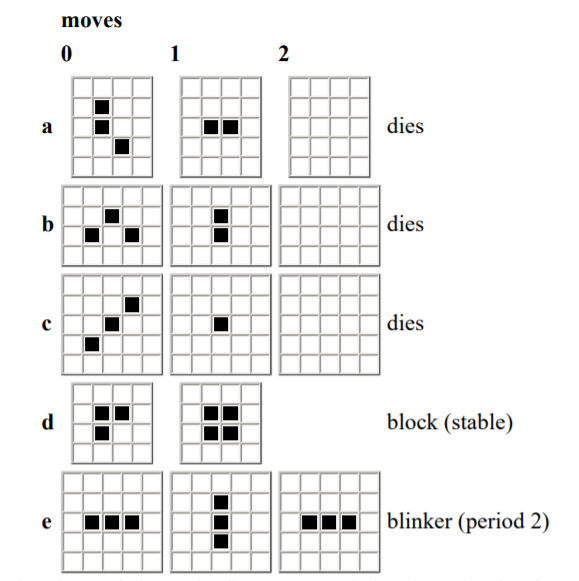
\includegraphics[width=\linewidth]{img/moves_1.png}
\caption{Evolution innerhalb von drei Generationen (entnommen aus \cite{gardner1970mathematical})}
\label{moves_1}
\end{figure}
In Abbildung \ref{moves_2} führen die Startmuster zu einem sogenannten "`beehive"', welches in dieser Position verharrt.
\begin{figure}[H]
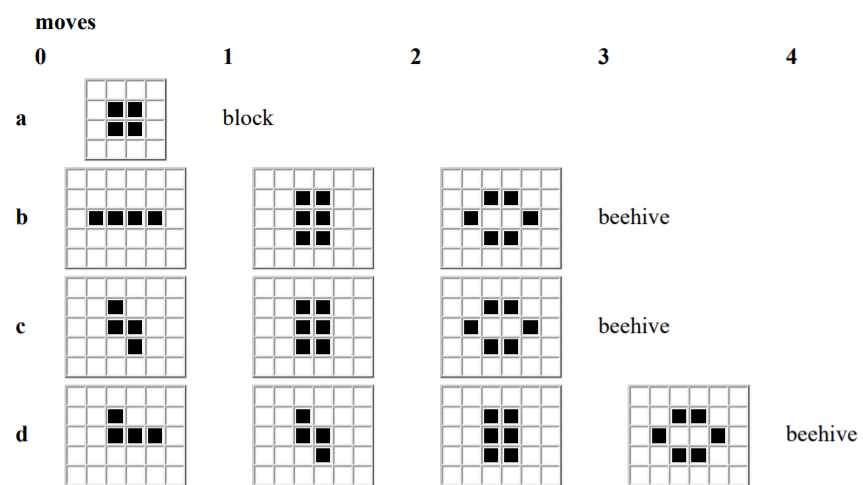
\includegraphics[width=\linewidth]{img/moves_2.png}
\caption{Evolution innerhalb von vier Generationen (entnommen aus \cite{gardner1970mathematical})}
\label{moves_2}
\end{figure}

\paragraph{Implementierung}

Für die Implementierung des Algorithmus wurden folgende Parameter gewählt:
\begin{itemize}
\item Anzahl der Spalten und Reihen des Gitters: Es wird eine Zahl angegeben, durch die die Weite und Breite des Gitters geteilt wird. So ergibt sich dann die Anzahl der Spalten und Reihen.
\item Farbe für den Vorgang der Reproduktion: Immer wenn eine Zelle geboren wird, wird sie für diese Runde in dieser Farbe angezeigt.
\item Farbe für den Vorgang des Sterbens: Immer wenn eine Zelle stirbt, wird sie für diese Runde in dieser Farbe angezeigt.
\end{itemize}
Wobei die Farbe für tote Zellen immer transparent und die Farbe für lebende Zellen immer schwarz ist. Die Startwerte für das Gitter werden anhand des vorhergehenden Algorithmus oder, sollte dies der erste Algorithmus sein, zufällig anhand eines Seeds gewählt. Nach dem Start beginnt das Spiel des Lebens und kann beispielsweise nachfolgende Bilder ergeben. Die nächsten vier Bilder zeigen die Evolution eines acht mal acht Gitter (hellblau = sterben, hellgrün = geboren werden). Die Bildschirmbreite und -höhe wurde bei 1000 Pixeln festgesetzt, welche wiederum durch 120 geteilt wurde, um die Spalten- bzw. Reihenanzahl zu erhalten.

\begin{figure}[H]
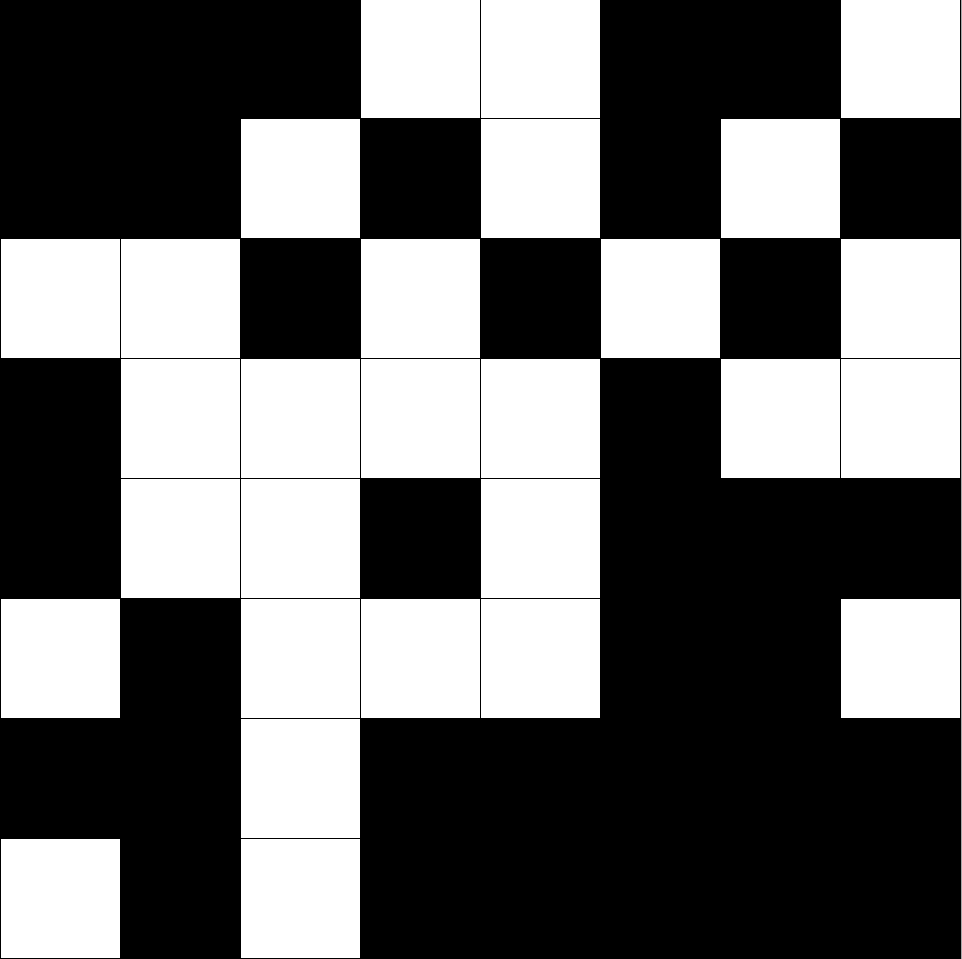
\includegraphics[width=5cm]{img/8x8_start.png}
\caption{Startzustand des 8x8-Gitters (eigene Darstellung)}
\label{8x8_start}
\end{figure}

\begin{figure}[H]
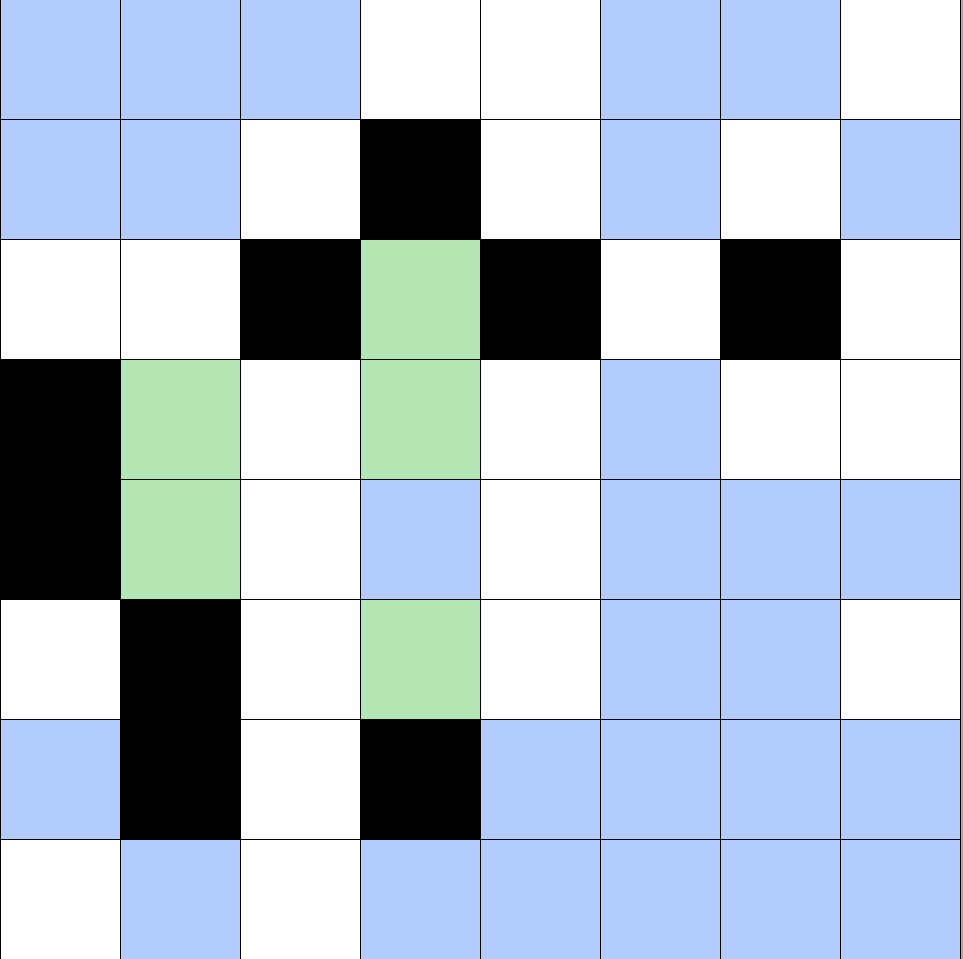
\includegraphics[width=5cm]{img/8x8_firstgen.png}
\caption{Die erste Generation (eigene Darstellung)}
\label{8x8_firstgen}
\end{figure}

\begin{figure}[H]
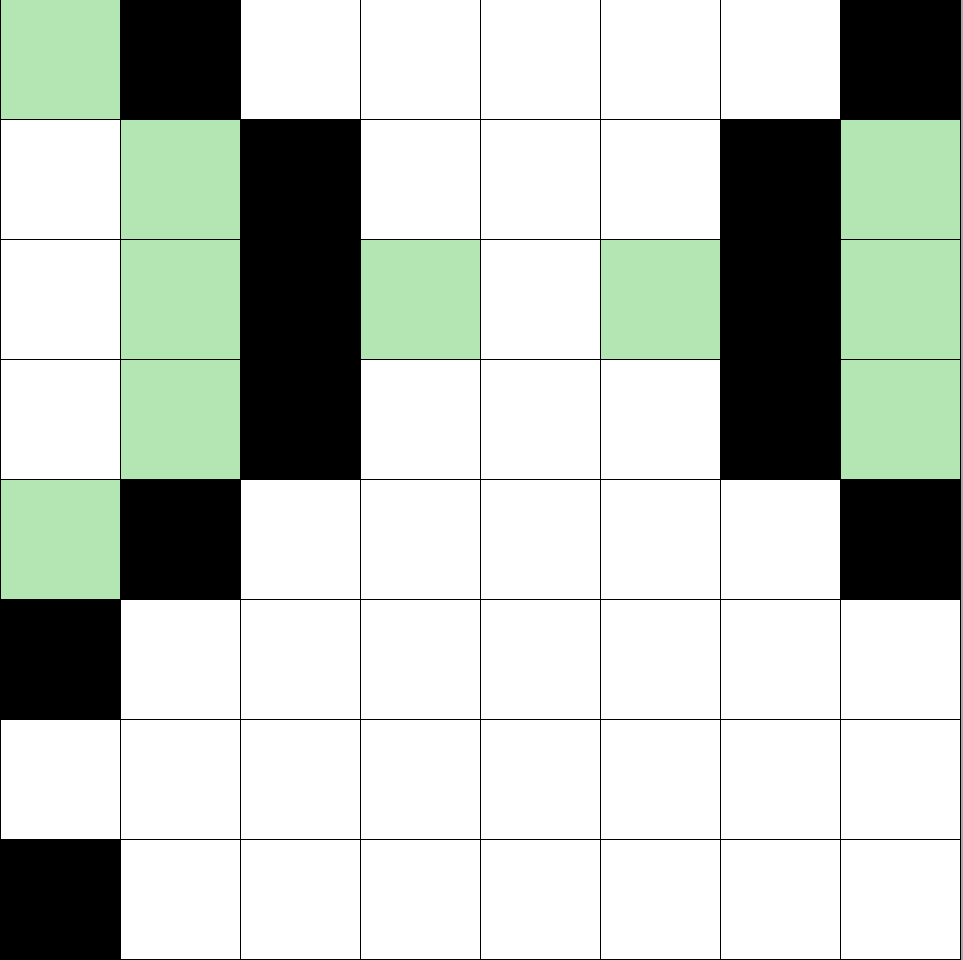
\includegraphics[width=5cm]{img/8x8_gen16.png}
\caption{16. Generation: Achsensymmetrisches (fast punktsymmetrisches) Objekt (eigene Darstellung)}
\label{8x8_gen16}
\end{figure}

\begin{figure}[H]
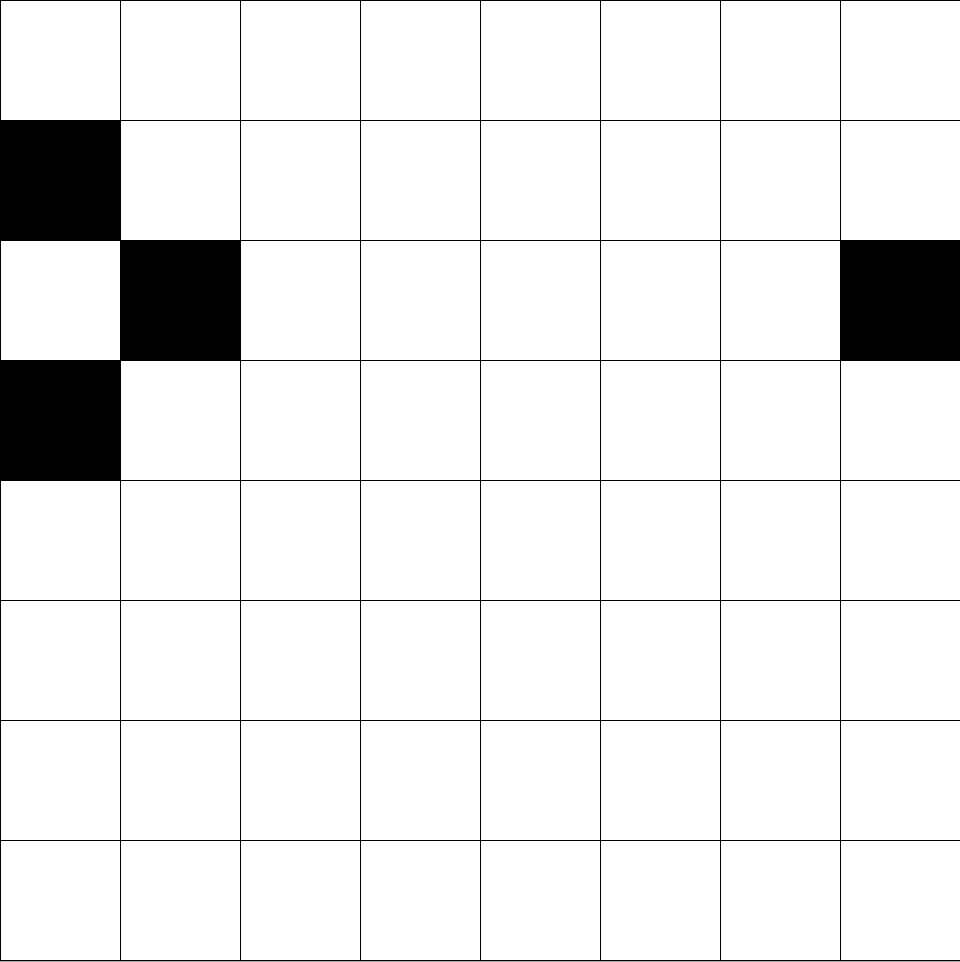
\includegraphics[width=5cm]{img/8x8_final.png}
\caption{Endzustand des 8x8-Gitters (eigene Darstellung)}
\label{8x8_final}
\end{figure}

Die nächsten fünf Bilder zeigen die Evolution eines 12 mal 12 Gitters (blau = sterben, grün = geboren werden), wobei diese Konfiguration zum Aussterben aller Zellen nach 45 Generationen führt. Die Bildschirmbreite und -höhe wurde bei 1000 Pixeln festgesetzt, welche wiederum durch 80 geteilt wurde, um die Spalten- bzw. Reihenanzahl zu erhalten.

\begin{figure}[H]
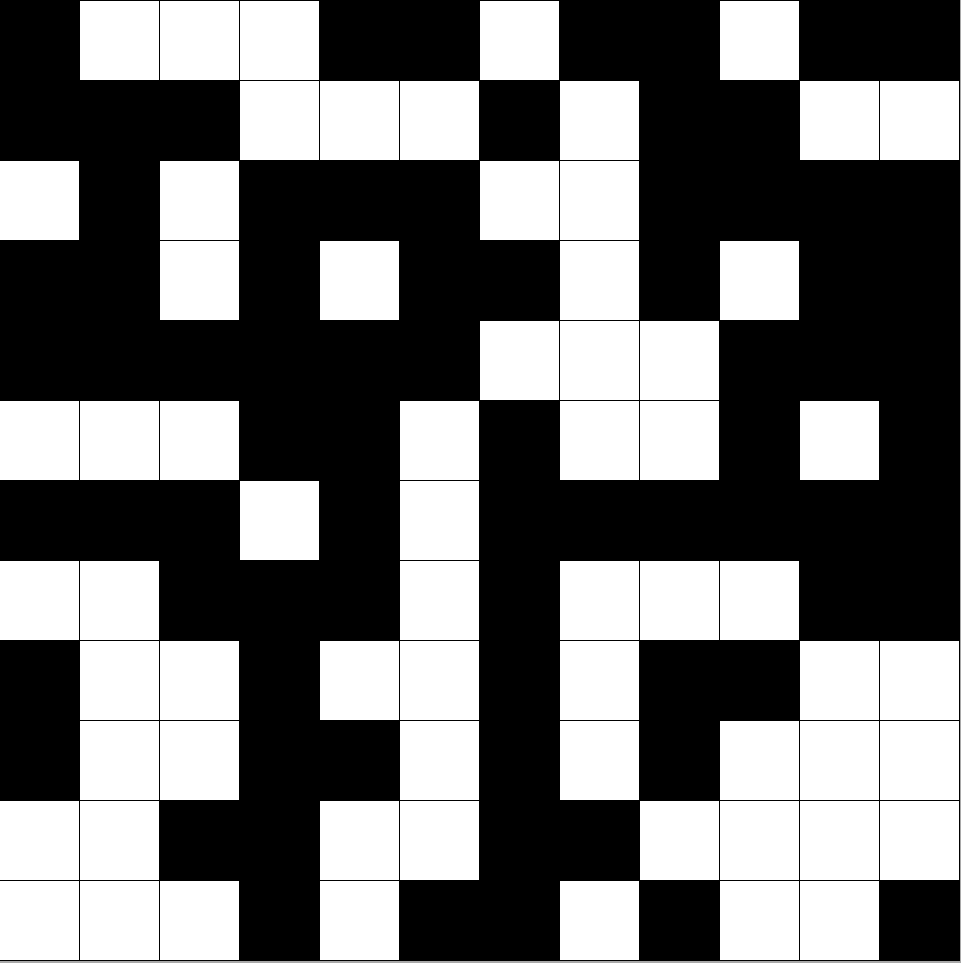
\includegraphics[width=5cm]{img/12x12_start.png}
\caption{Startzustand des 12x12-Gitters (eigene Darstellung)}
\label{12x12_start}
\end{figure}

\begin{figure}[H]
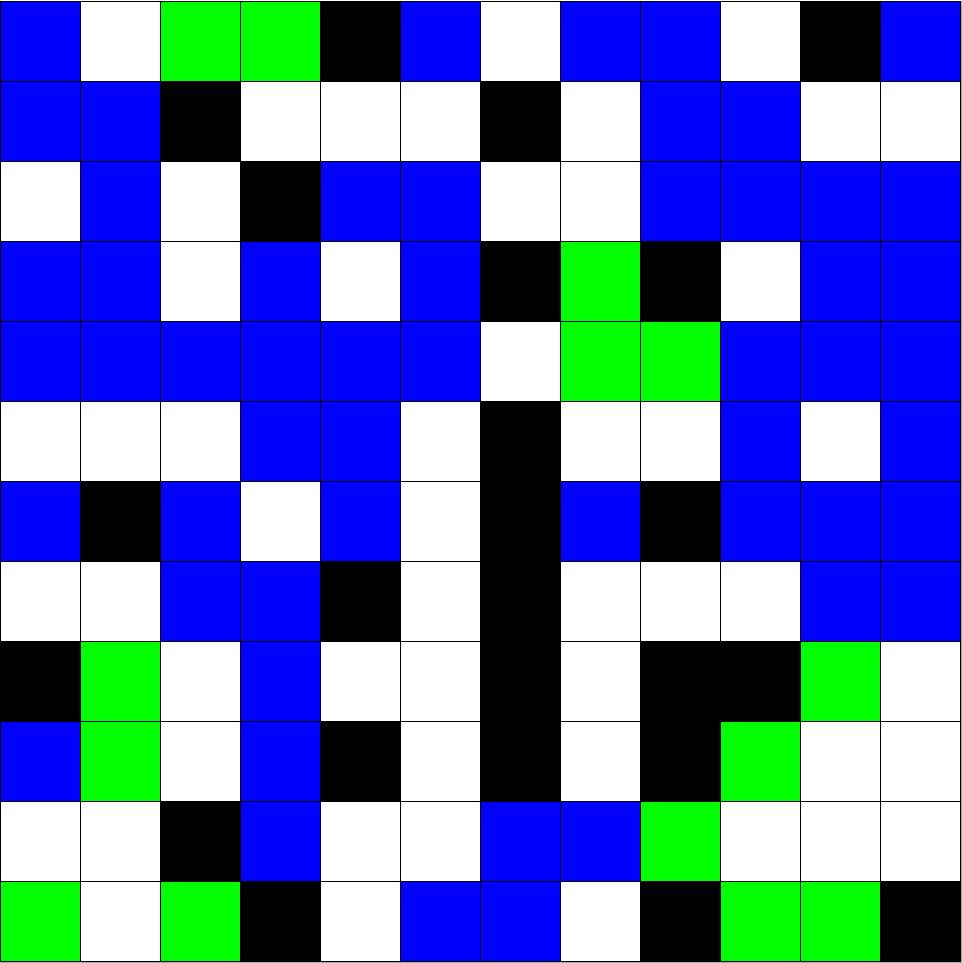
\includegraphics[width=5cm]{img/12x12_firstgen.png}
\caption{Die erste Generation (eigene Darstellung)}
\label{12x12_firstgen}
\end{figure}

\begin{figure}[H]
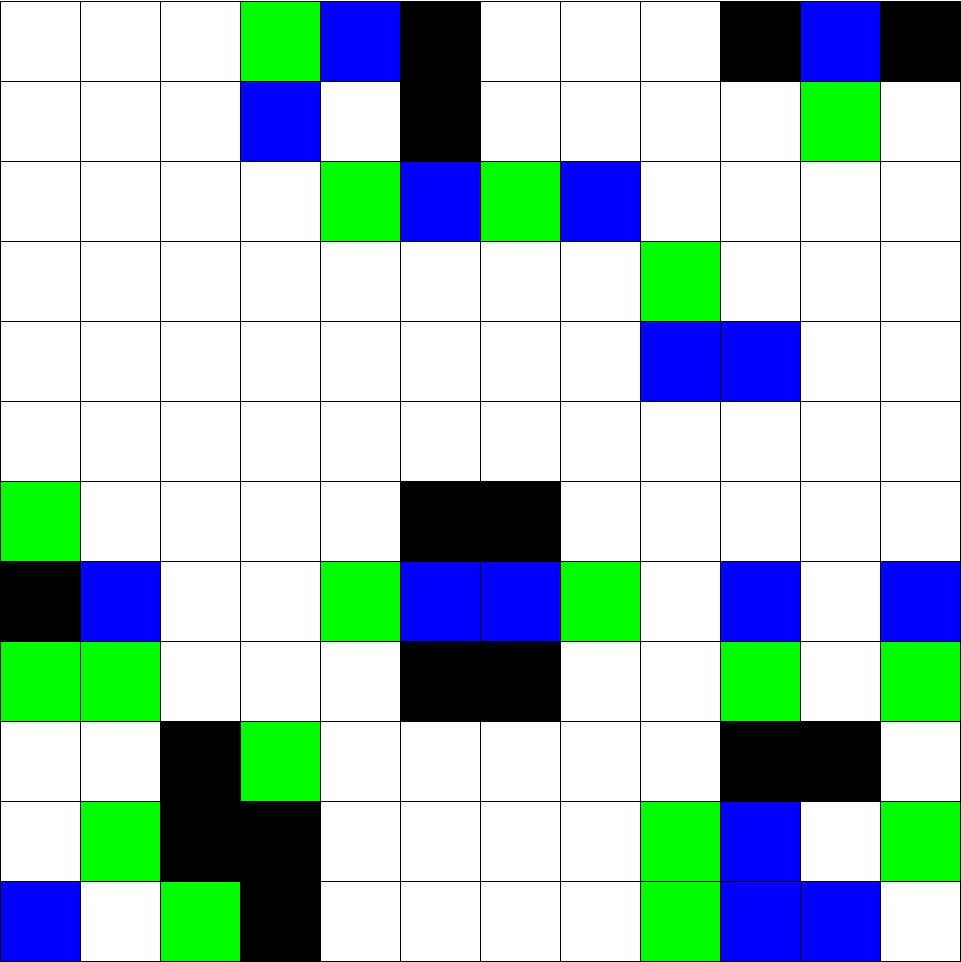
\includegraphics[width=5cm]{img/12x12_gen4.png}
\caption[Vierte Generation: Sechser Block]{Vierte Generation: Hier führt ein Sechser-Block zu einem beehive in der nächsten Generation (eigene Darstellung, vgl. Abbildung \ref{moves_2})}
\label{12x12_gen4}
\end{figure}

\begin{figure}[H]
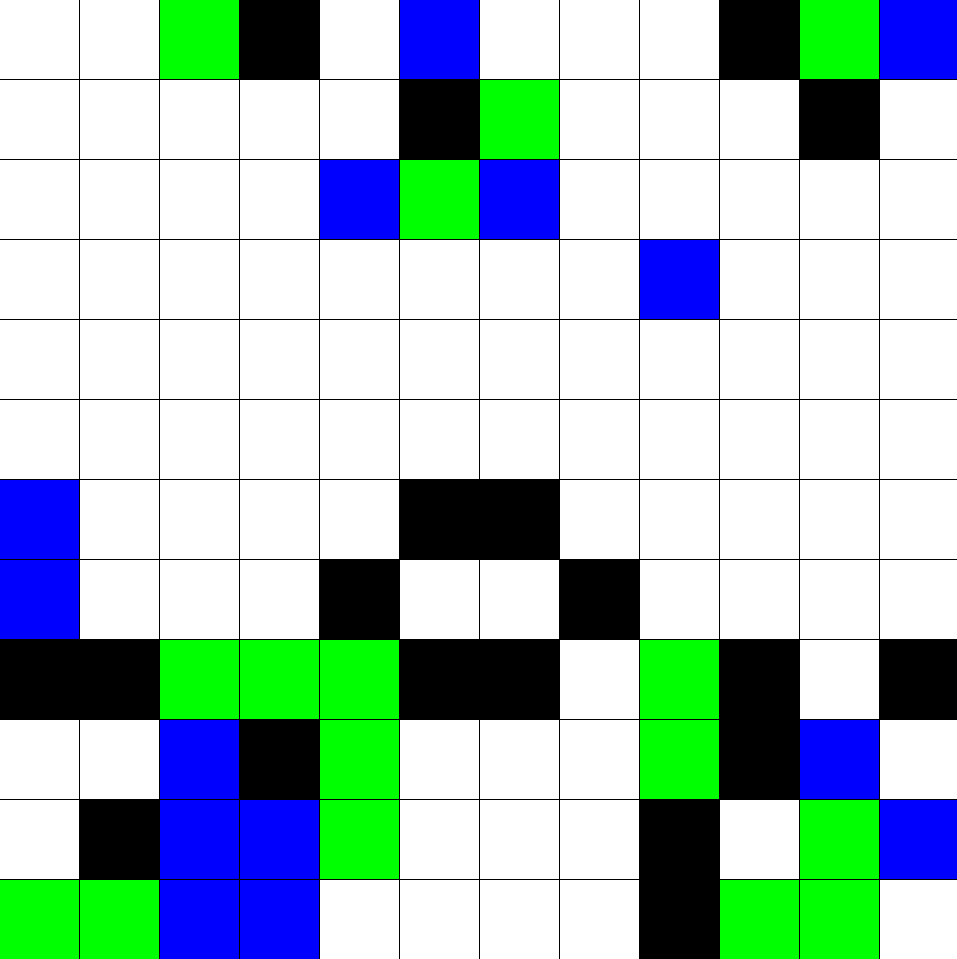
\includegraphics[width=5cm]{img/12x12_beehive_gen5.png}
\caption{Fünfte Generation: Es entstand ein beehive (eigene Darstellung)}
\label{12x12_beehive_gen5}
\end{figure}

\begin{figure}[H]
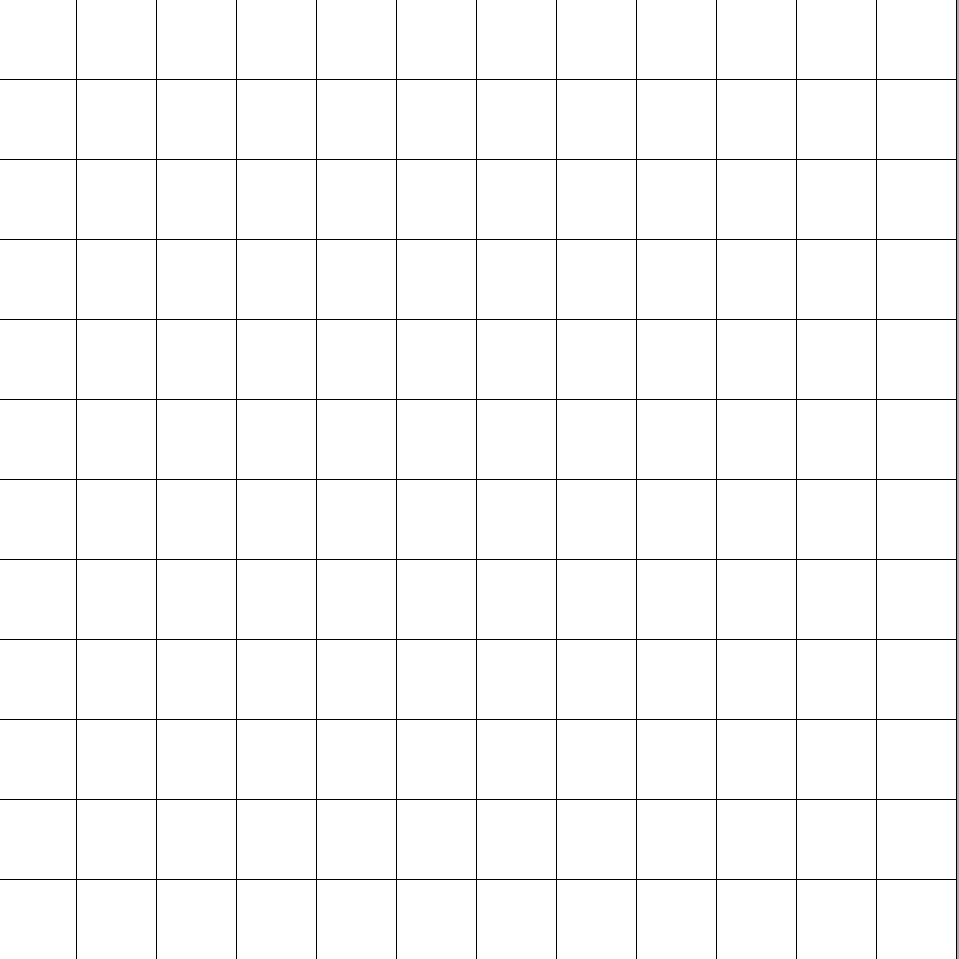
\includegraphics[width=5cm]{img/12x12_empty_gen45.png}
\caption{Endzustand des 12x12-Gitters: Alle Zellen sind gestorben (eigene Darstellung)}
\label{12x12_empty_gen45}
\end{figure}

Nach etlichen Generationen endet nachfolgendes Game of Life in vier Blinkern. Es handelt sich um ein zehn mal zehn Gitter. Die Konfiguration kann den Beispielen im Konfigurator entnommen werden.

\begin{figure}[H]
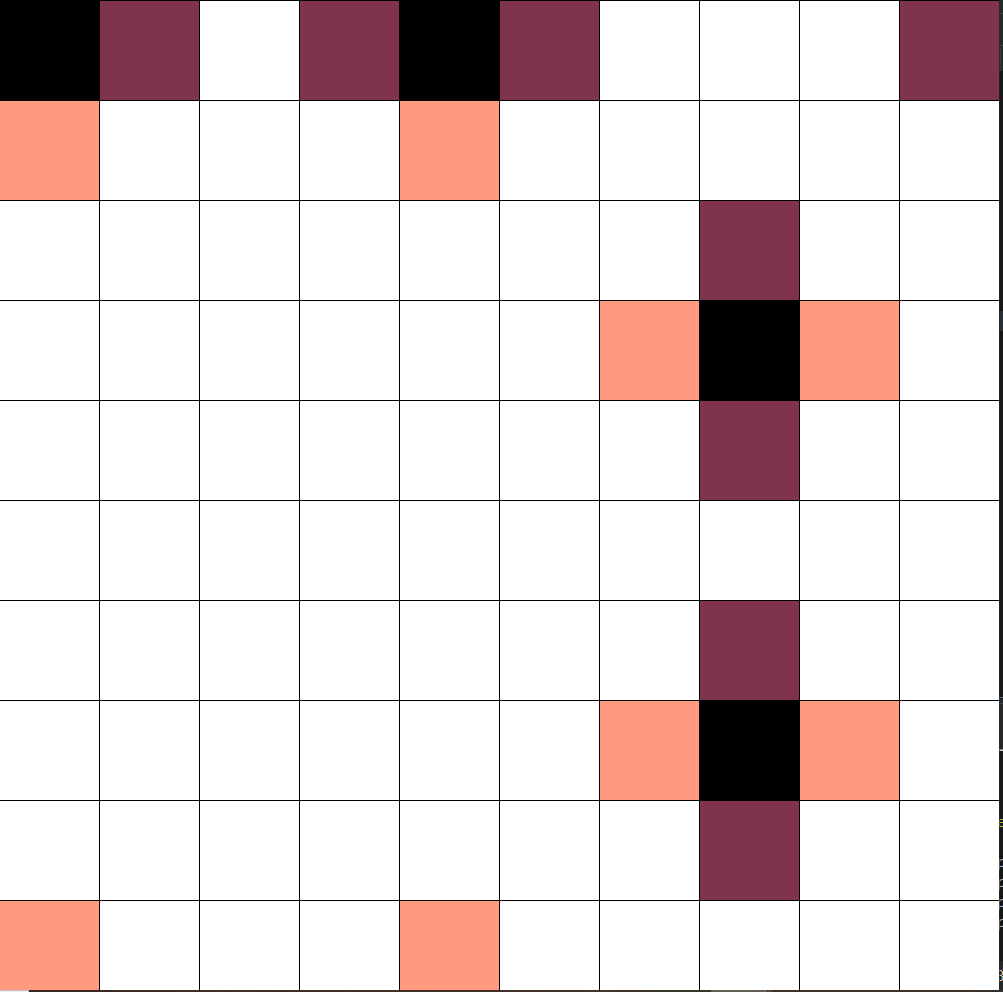
\includegraphics[width=5cm]{img/10x10_blinker_seed10000.png}
\caption{10x10 Gitter: Blinker 1 (eigene Darstellung)}
\label{10x10_blinker_seed10000}
\end{figure}

\begin{figure}[H]
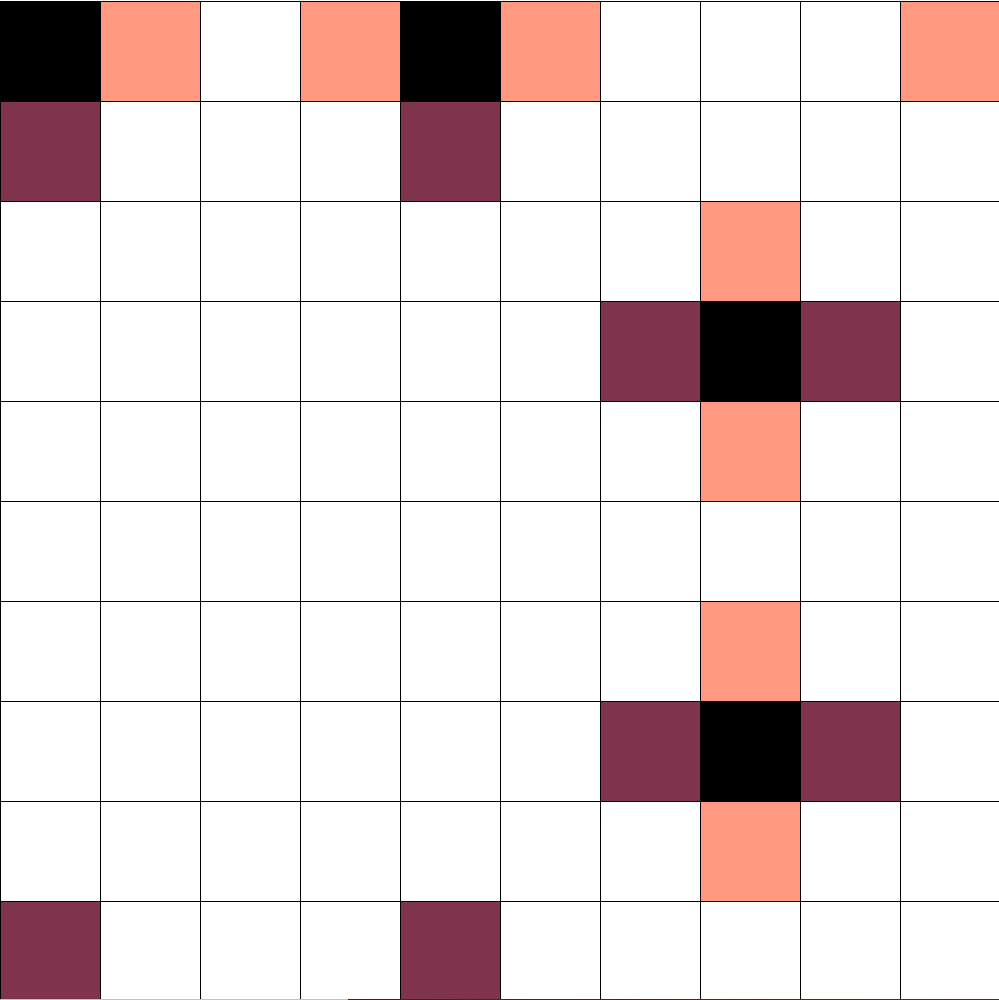
\includegraphics[width=5cm]{img/other_10x10_blinker_seed10000.png}
\caption{10x10 Gitter: Blinker 2 (eigene Darstellung)}
\label{other_10x10_blinker_seed10000}
\end{figure}

\paragraph{Bewertung}
Das Beobachten der Evolution mithilfe des Game of Life Algorithmus macht Spaß. Dabei lässt sich die Stärke des Algorithmus ebenso als seine Schwäche bezüglich der Kooperation benennen. Der Algorithmus braucht nicht unbedingt eine Kooperation um schöne Bilder zu erzeugen. Er ist in sich schon sehr vielfältig, was dazu führt dass viele unterschiedliche Bilder entstehen. Des Weiteren ist der Algorithmus zunächst einmal im Rahmen seines Gitters eingeschränkt, eine Erweiterung auf 3D oder andere geometrische Objekte wäre sicher spannend. Je nachdem, wie der Startzustand des Algorithmus ist, kann auch ein leeres Bild entstehen, sofern alle Zellen gestorben sind. Der Algorithmus lebt von seiner Ausführung und weniger von dessen Endzustand. Der GOL kann unter Umständen sehr lange laufen, oder auch nur kurz. 


\subsubsection{L-System}

Das Lindenmayer-System bzw. L-System wurde 1968 von einem Biologen desselben Namens eingeführt. Es handelt sich um eine mathematische Theorie über die Entwicklung von (oft pflanzlichen) rekursiven Systemen. Für ein L-System werden also Regeln benötigt, die zur Generierung der Systeme herangezogen werden. Ein einführendes Axiom verzeichnet den Beginn der Entwicklung und die Regeln werden dann rekursiv angewendet \cite{wiki2018lsystem}. Es werden demnach nachfolgende Teilaspekte benötigt:
\begin{itemize}
\item Alphabet: Definition der Zeichen, die erlaubt sind.
\item Axiom: Definition des Beginns des Systems.
\item Regelsatz: Vorgabe der Regeln, welche rekursiv angewandt werden.
\end{itemize}
Zur besseren Darstellung soll ein einfaches Beispiel herangezogen werden:
\begin{itemize}
\item Alphabet: A und B,
\item Axiom: A,
\item Regelsatz: Aus A wird AB, aus B wird BB.
\end{itemize}
In Tabelle \ref{tab:l-system-beispiel} wird die rekursive Entwicklung dargestellt.

\begin{table}[H]
\begin{tabular}{@{}|l|l|l|l|l|@{}}
\toprule
\textbf{Axiom} & \textbf{Gen1} & \textbf{Gen2} & \textbf{Gen3} & \textbf{...} \\ \midrule
A              & AB            & ABBB          & ABBBBBBB      & ...          \\ \bottomrule
\end{tabular}
\caption{Anhand des Regelsatzes wird das Axiom rekursiv erweitert.}
\label{tab:l-system-beispiel}
\end{table}

Es wird schnell klar, dass der Algorithmus ohne Abbruchbedingung unendlich weiter laufen würde bzw. nur durch die Rechenleistung begrenzt ist. Wie kann dieser Algorithmus nun für eine grafische Darstellung genutzt werden? 

\paragraph{Implementierung}
Zur grafischen Umsetzung, muss den Regelsätzen eine andere Bedeutung gegeben werden. Dem Benutzenden der grafischen Oberfläche sollen die Wahl des x- und y-Startpunktes sowie der Farbe und verschiedene Regelsätze zur Verfügung gestellt werden. Die Regelsätze orientieren sich an Ihren Erfindern und heißen im Einzelnen:
\begin{itemize}
\item Verästelung,
\item Koch,
\item Fractal,
\item Sierpinksi Gasket Triangle und
\item Überraschung.
\end{itemize}
Beispielhaft soll auf drei davon im Folgenden eingegangen werden. Zunächst wird die "`Verästelung"' beschrieben:
\begin{itemize}
\item Alphabet: F = ein Stück zeichnen, [ = abspeichern, ] = auslesen, + = Drehung gegen den Uhrzeigersinn, - = Drehung im Uhrzeigersinn (jeweils um 45°, bzw. abhängig vom Seed)
\item Axiom: F-F-F-F
\item Regelsatz: Aus "`F"' wird "`F[F]-F+F[--F]+F-F"'
\end{itemize}

In Abbildung \ref{veraestelung_gen5} wird eine besonders schöne Verästelung dargestellt. In Abbildung \ref{gespiegelter_baum_gen6} wird mit Spiegelung gearbeitet.
\begin{figure}[H]
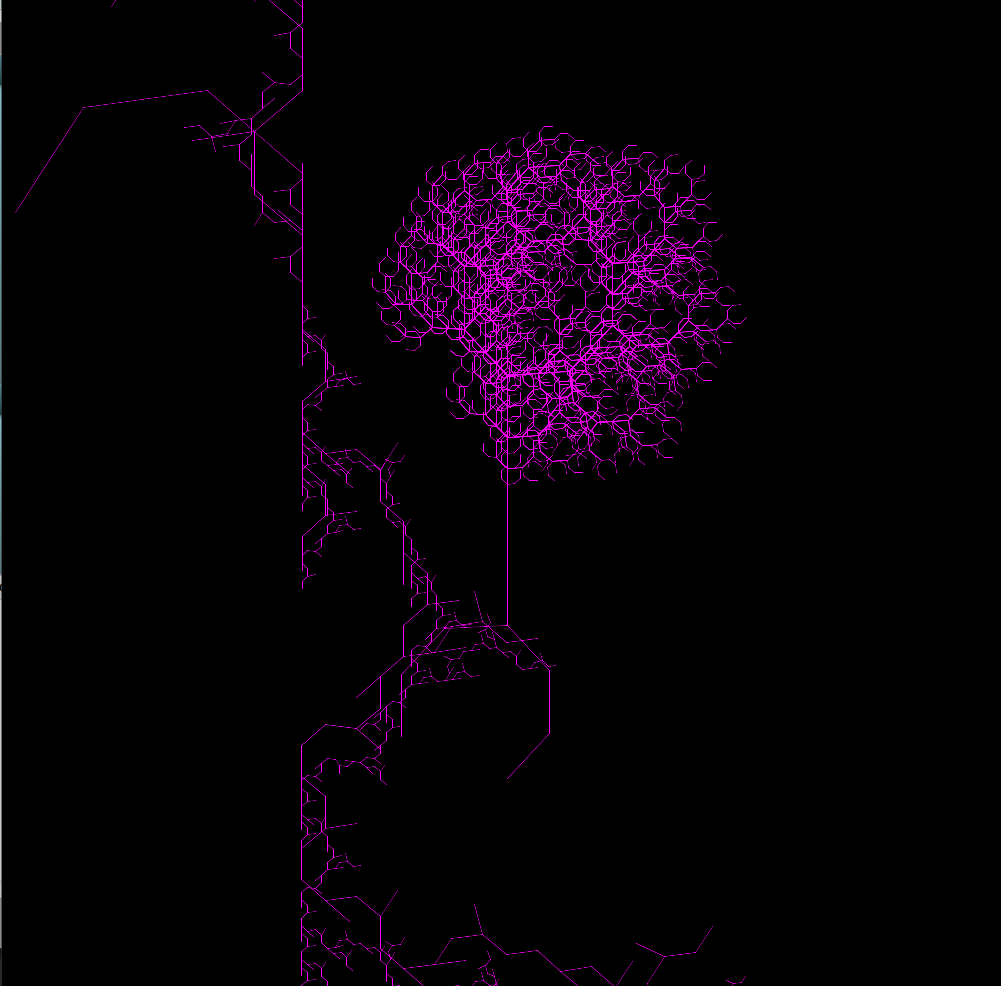
\includegraphics[width=10cm]{img/veraestelung_gen5.png}
\caption{Fünfte Generation: Ein Baum und weitere Verästelungen (eigene Darstellung)}
\label{veraestelung_gen5}
\end{figure}

\begin{figure}[H]
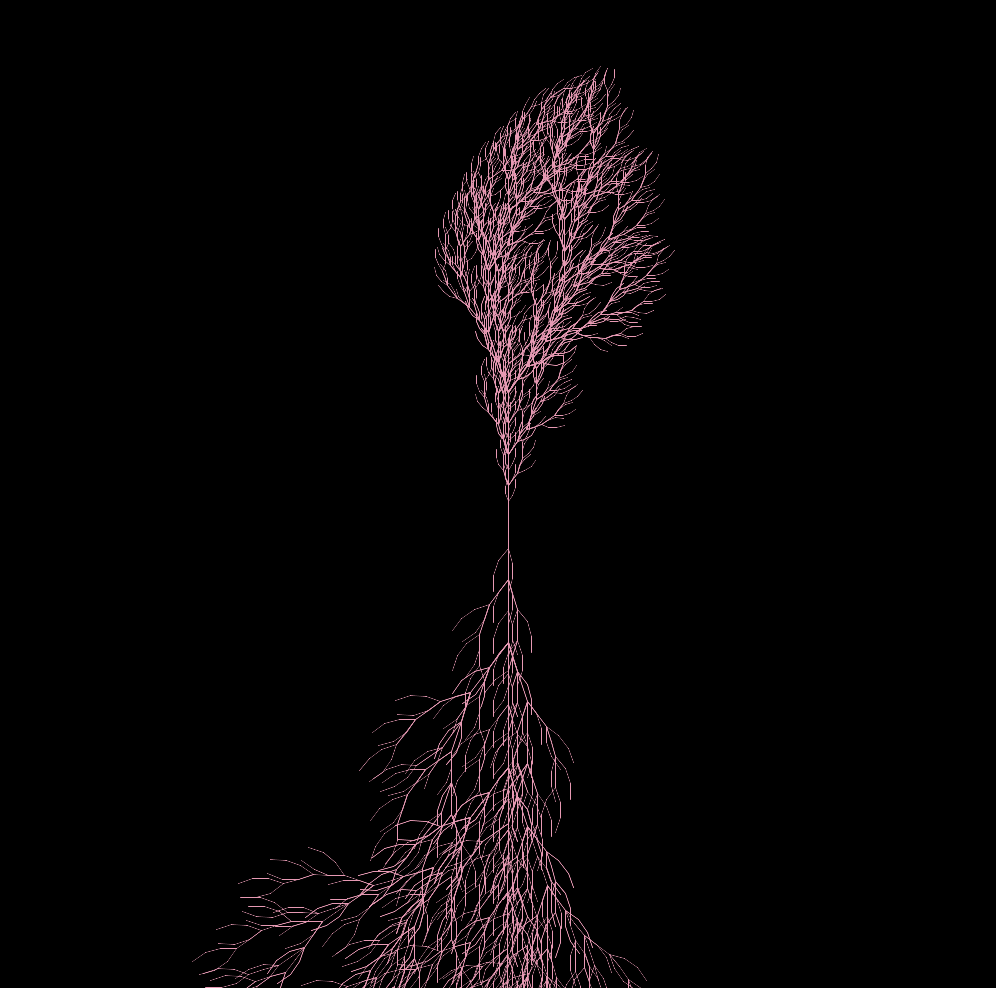
\includegraphics[width=10cm]{img/gespiegelter_baum_gen6.png}
\caption{Sechste Generation: Der Baum zeichnet abwechselnd nach oben und unten (eigene Darstellung)}
\label{gespiegelter_baum_gen6}
\end{figure}

Als zweite Kategorie der L-Systeme soll "`Fractal"' vorgestellt werden. 
\begin{itemize}
\item Alphabet: F = ein Stück zeichnen, + = Drehung gegen den Uhrzeigersinn, - = Drehung im Uhrzeigersinn (jeweils um 90°, bzw. abhängig vom Seed)
\item Axiom: F-F-F-F
\item Regelsatz: Aus "`F"' wird "`FF-F-F-F-F-F+F"'
\end{itemize}
Die Abbildungen \ref{fractal-gen5} bis \ref{fractal-gen5-grad} zeigen einige Fraktale. Fraktale sind natürliche oder künstliche, meist geometrische Muster, die eine gebrochene Hausdorff-Dimension besitzen. Daher kommt auch der Name. Sie weisen eine hohe Selbstähnlichkeit auf, wenn sie zum Beispiel aus kleineren Kopien von sich selbst bestehen \cite{mandelbrot1983fractal}. Der Algorithmus macht also viele kleinere Kopien von sich selbst und wird dabei um eine gewisse Gradzahl gedreht. Werden die Gradzahlen angepasst, können komplett unterschiedliche Bilder entstehen.

\begin{figure}[H]
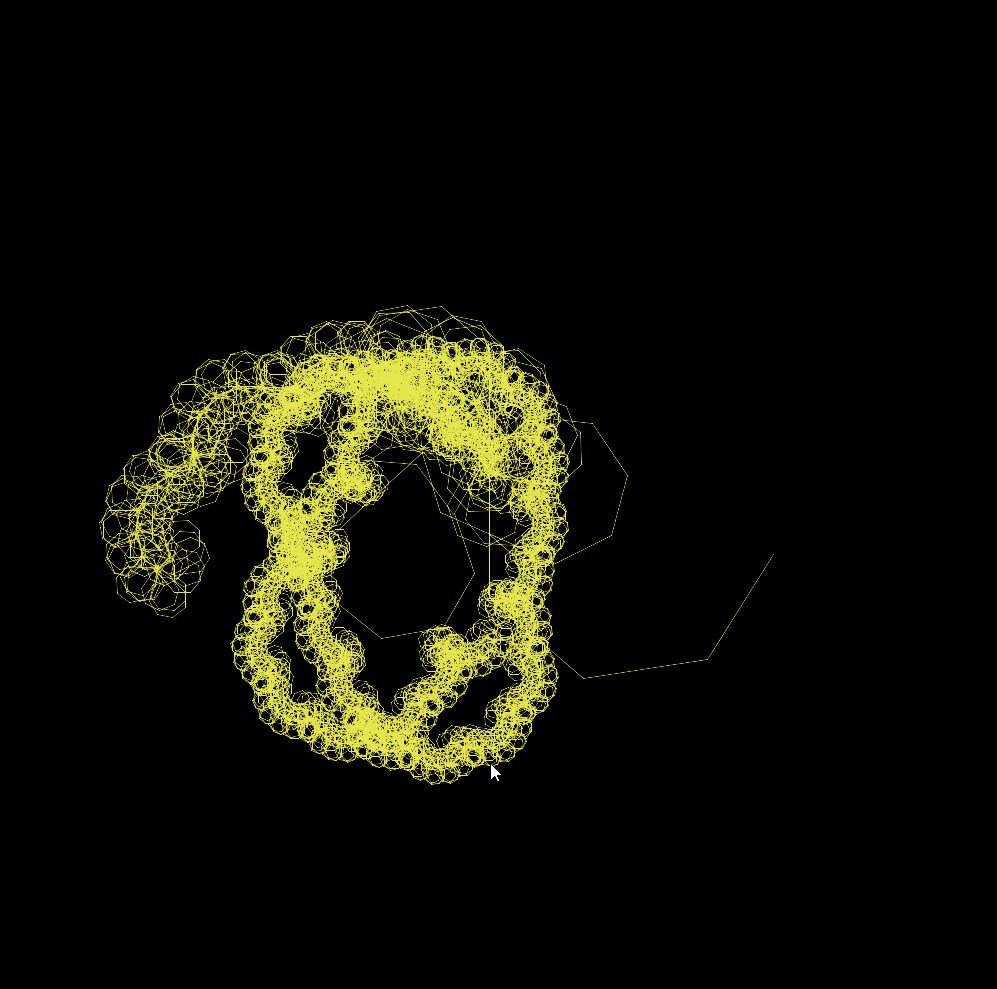
\includegraphics[width=10cm]{img/fractal-gen5.png}
\caption{Fünfte Generation: Eine wolkige Struktur (eigene Darstellung)}
\label{fractal-gen5}
\end{figure}

\begin{figure}[H]
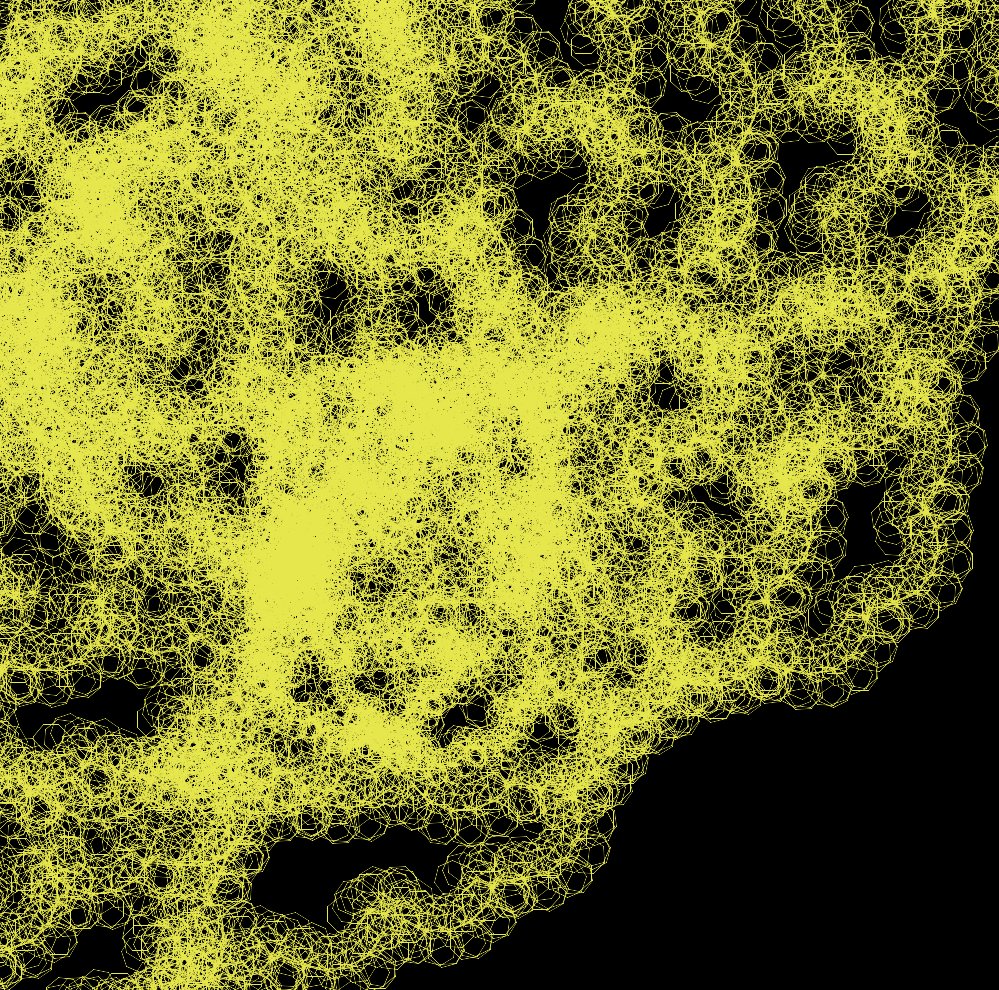
\includegraphics[width=10cm]{img/fractal-gen6.png}
\caption{Sechste Generation: Die Fraktale sind fast über das gesamte Bild verteilt (eigene Darstellung)}
\label{fractal-gen6}
\end{figure}

\begin{figure}[H]
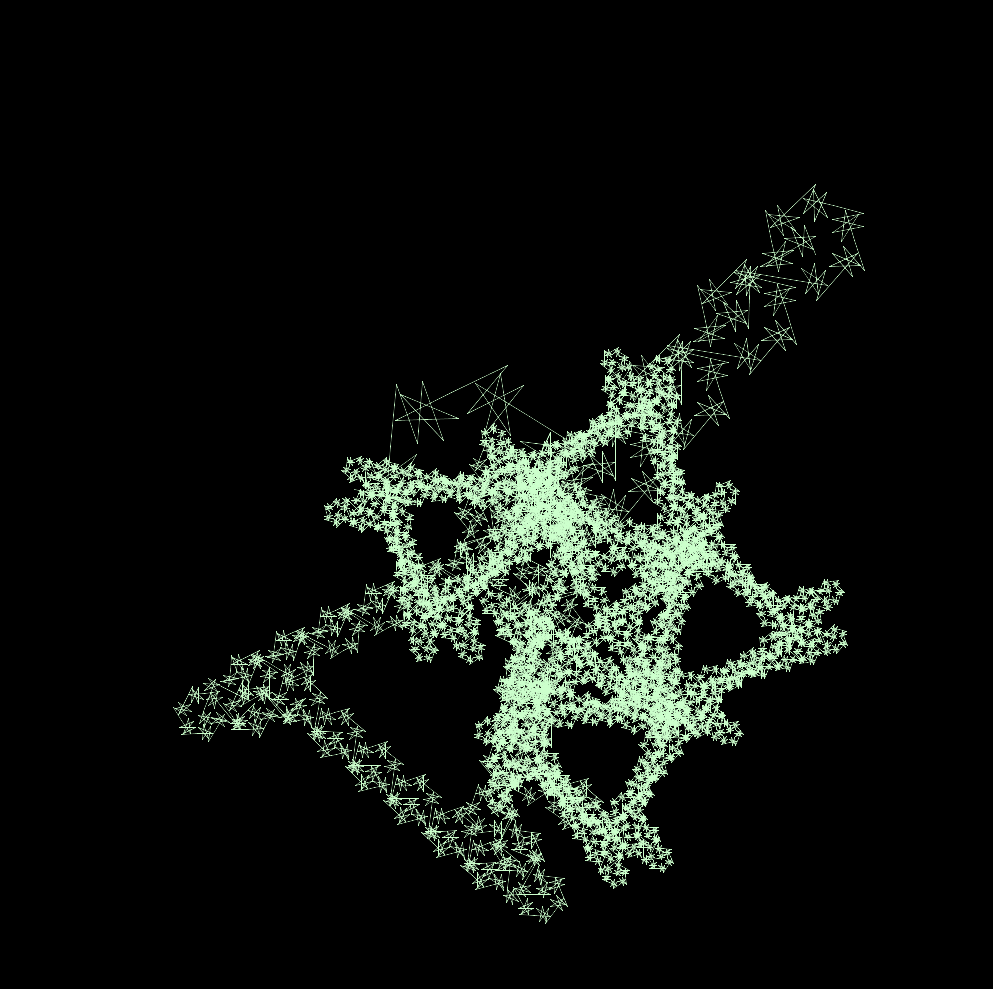
\includegraphics[width=10cm]{img/fractal-gen5-grad.png}
\caption[Fünfte Generation: Erhöhung der Gradzahl]{Fünfte Generation: Wird die Gradzahl erhöht, werden die Fraktale kantiger und erhalten eine Schneeflockenstruktur (eigene Darstellung)}
\label{fractal-gen5-grad}
\end{figure}

Zuletzt soll noch "`Sierpinski"' beschrieben werden. Hier enthält der Regelsatz zwei Regeln.
\begin{itemize}
\item Alphabet: F/G = ein Stück zeichnen, - = Drehung im Uhrzeigersinn (um 25°, bzw. abhängig vom Seed)
\item Axiom: F--F--F
\item Regelsatz: Aus "`F"' wird "`F--F--F--G"' und aus "`G"' wird "`GG"'
\end{itemize}

In den Abbildungen \ref{sierpinski-gen7} und \ref{sierpinski-gen10} wird "`Sierpinski"' in den Generationen sieben und zehn dargestellt. Der Algorithmus ist an der Sierpinski-Kurve orientiert.

\begin{figure}[H]
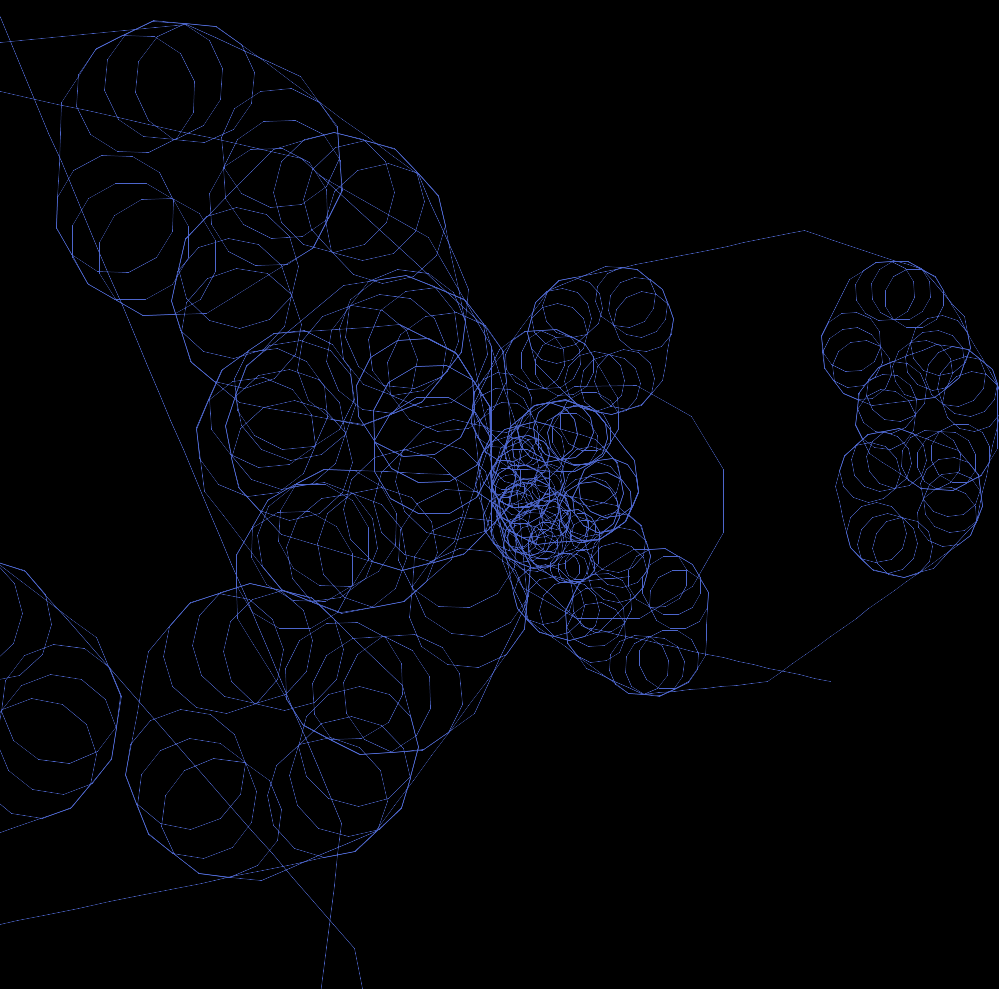
\includegraphics[width=10cm]{img/sierpinski-gen7.png}
\caption{Siebte Generation: Sieht einem Diamantring ähnlich (eigene Darstellung)}
\label{sierpinski-gen7}
\end{figure}

\begin{figure}[H]
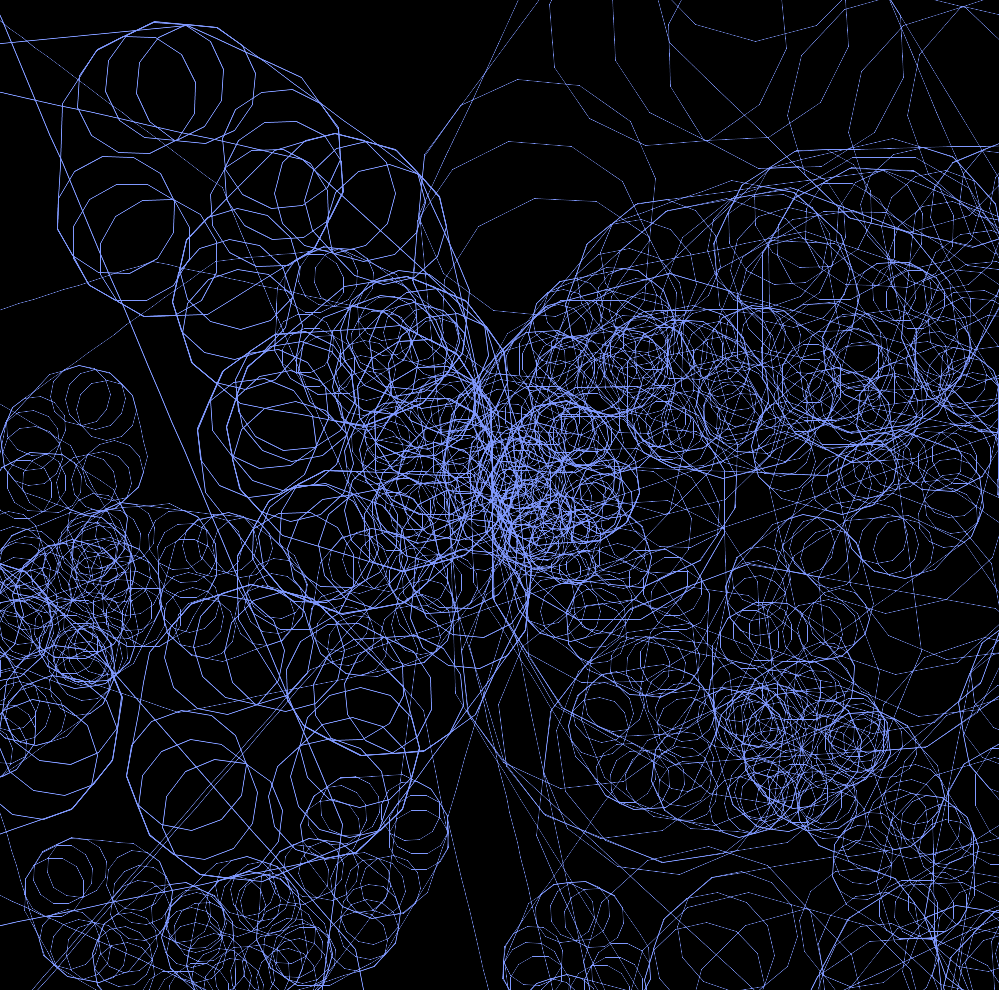
\includegraphics[width=10cm]{img/sierpinski-gen10.png}
\caption{Zehnte Generation: Endlose Spiralen (eigene Darstellung)}
\label{sierpinski-gen10}
\end{figure}

\paragraph{Bewertung}
Der Algorithmus bietet unendlich viele Möglichkeiten, um verschiedene geometrische Formen darzustellen. Der Fantasie sind dabei keine Grenzen gesetzt. So gestaltet es sich auch mit der Kooperation. Ein Baum kann dort entstehen, wo ein vorheriges Bild geendet hat oder ein Schwarm kann aus den letzten Verästelungen eines Baumes heraus fliegen. Darüber hinaus ist ein L-System meistens selbst schon so komplex und beeindruckend, dass eine räumliche Kooperation, sprich nebeneinander gelegte Bilder auch für sich selbst stehen können.
Dadurch, dass L-Systeme zunächst nicht abbrechend sind und immer komplexer werden, kann es zu einem hohen Speicherverbrauch bzw. einer Runtime-Exception kommen. Die Iterationen sollten deshalb beschränkt sein.


\subsubsection{Particle System}
Mithilfe eines Partikelsystems lassen sich mehrere Objekte als Gesamtsystem animieren. Wind oder Feuer könnten solche Systeme sein oder beeinflussen. Durch verschiedene Parameter lassen sich die Partikel dann beeinflussen \cite{reeves1983particle}.


\paragraph{Implementierung}
Bei der Implementierung des Algorithmus diente \cite{shiffman2022smoke} als Vorlage. Es werden vier Bilder geladen (also durch den Nutzenden ausgewählt), welche dann von der Mitte des Bildes nach außen getrieben werden. Streng genommen handelt es sich also um vier Partikelsysteme. Das funktioniert, indem jeder neue Partikel der erstellt wird, die Optik des geladenen Bildes übernimmt. Die Windstärke wird vom vorherigen Algorithmus beeinflusst. Nach der Initialisierung der Systeme werden neue Partikel immer nur am Rand der Systeme hinzugefügt, zu dem der Wind sie treibt.
Beispiele können den Abbildungen \ref{black_materia_gen20} bis \ref{all_black} entnommen werden.

\begin{figure}[H]
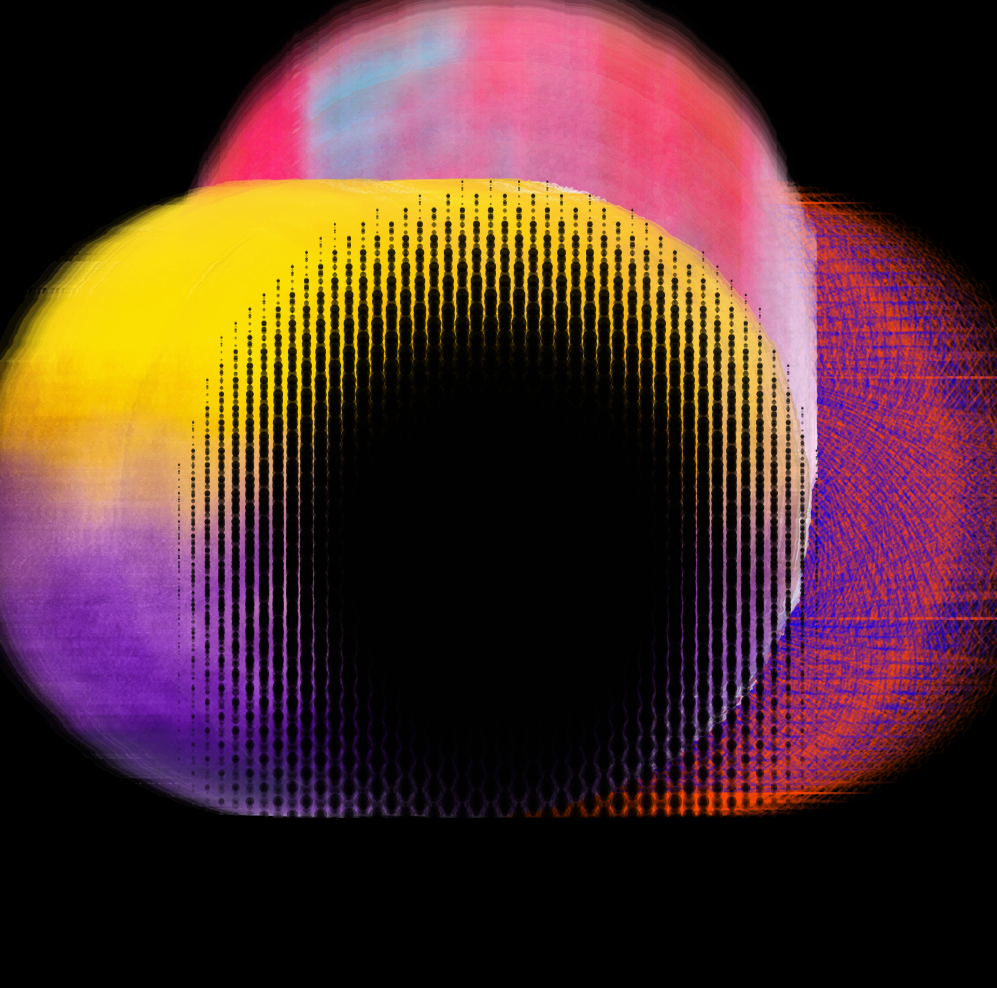
\includegraphics[width=10cm]{img/black_materia_gen20.png}
\caption{20. Generation: Schwarze Materie (eigene Darstellung)}
\label{black_materia_gen20}
\end{figure}

\begin{figure}[H]
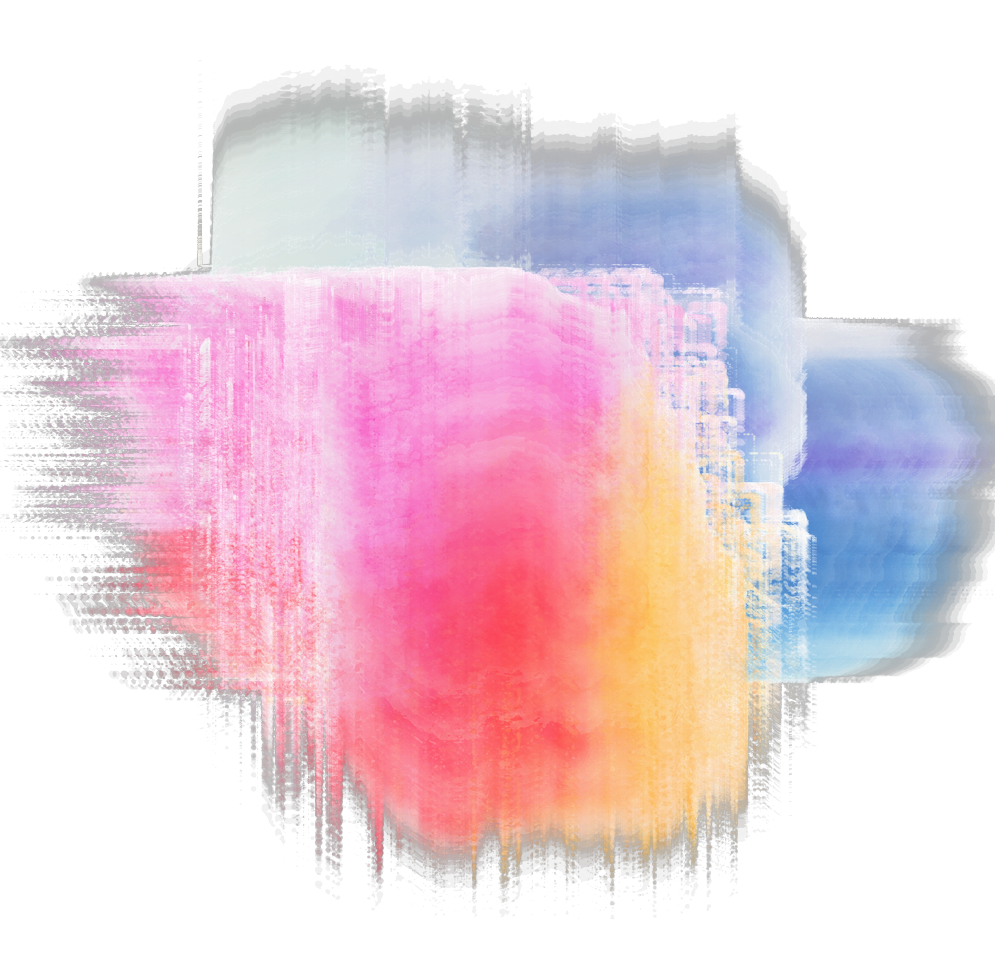
\includegraphics[width=10cm]{img/watercolor_gen20.png}
\caption{20. Generation: Wasserfarben werden über den Bildschirm verteilt (eigene Darstellung)}
\label{watercolor_gen20}
\end{figure}

\begin{figure}[H]
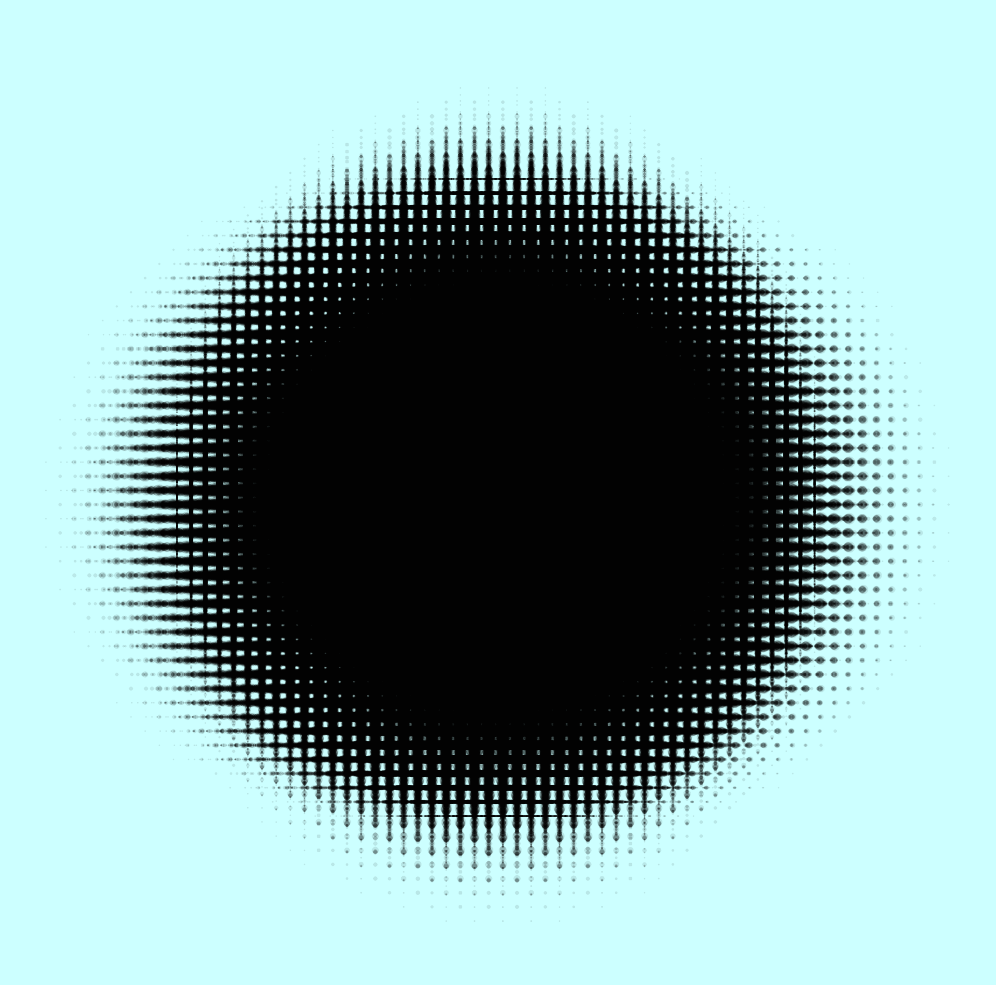
\includegraphics[width=10cm]{img/all_black.png}
\caption{Zehnte Generation: Die schwarzen Punkte verteilen sich (eigene Darstellung)}
\label{all_black}
\end{figure}

\paragraph{Bewertung}
Der Algorithmus hängt stark von den geladenen Bilder ab. Es ist daher von Vorteil, wenn ähnliche Bildstrukturen geladen werden, die auch ineinander verschwimmen können. Prinzipiell sind dadurch dem Erzeugen der Bilder und der Kreativität keine Grenzen gesetzt. 
Sofern der Algorithmus als erstes geladen wird, eignet er sich gut als Hintergrund für die darauffolgenden Algorithmen. Besonders nachfolgende Algorithmen, die anhand der vorherigen Farben beeinflusst werden funktionieren in dieser Verbindung gut. Räumliche Kooperationen funktionieren auch. Sollte der Algorithmus nicht als erstes geladen werden, überlagert er andere Bilder und eignet sich deshalb weniger. Nach etwa 30 Generationen wird der Speicherverbrauch relativ hoch. Die Iterationsanzahl sollte also begrenzt werden.

\subsubsection{Kooperation der eigenen Algorithmen}
Im Konfigurator lassen sich drei unterschiedliche Kooperationsmodi auswählen. Zunächst wird in Abbildung \ref{l_gol_p_l_gen5_nebeneinander} der Kooperationsmodus "`Nebeneinander 2x2"' dargestellt. Das Bild besteht von links oben nach rechts unten aus:
\begin{itemize}
\item LSystem: Fractal
\item Game of Life
\item Particle System
\item LSystem: Überraschung
\end{itemize}

\begin{figure}[H]
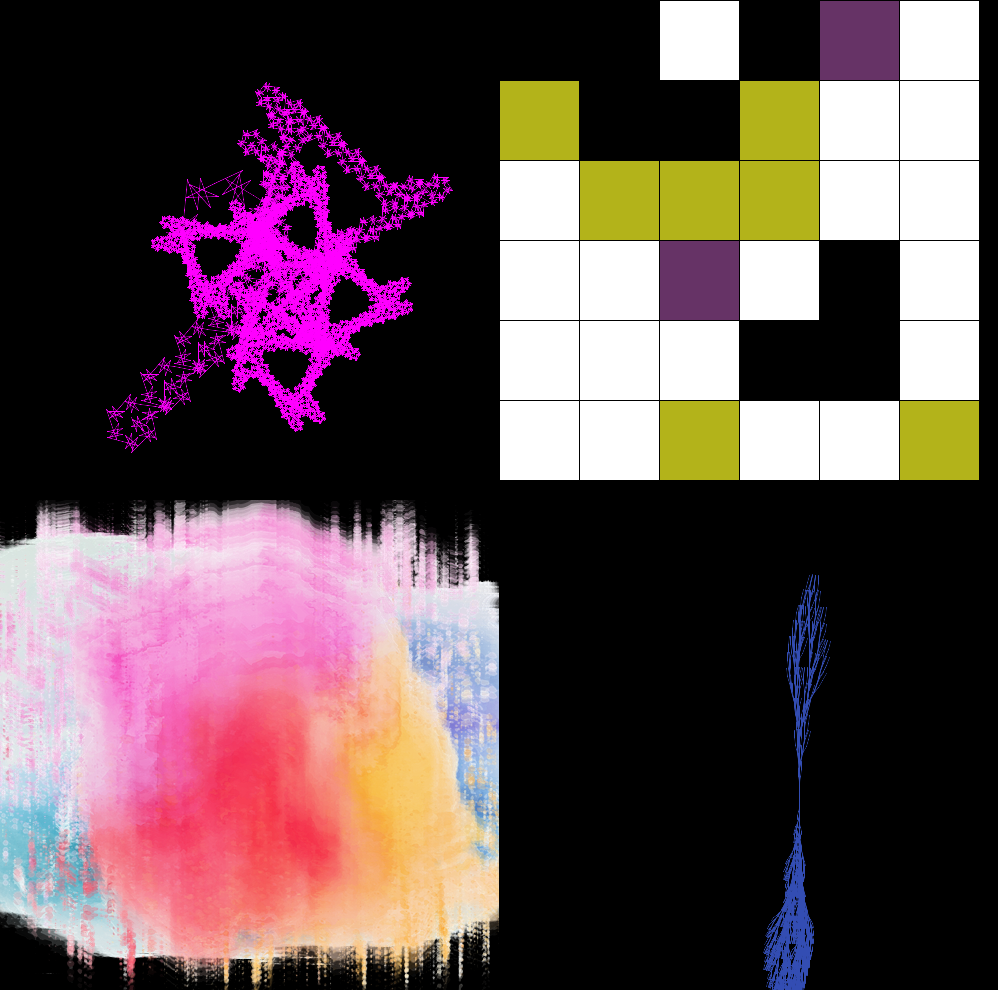
\includegraphics[width=\linewidth]{img/l_gol_p_l_gen5_nebeneinander.png}
\caption[Räumliche Trennung]{Fünfte Generation: Die vier Algorithmen werden räumlich getrennt voneinander ausgeführt (eigene Darstellung)}
\label{l_gol_p_l_gen5_nebeneinander}
\end{figure}

Als Nächstes wird in Abbildung \ref{sierpinski_veraestelung_gen8_nebeneinander2x1} der Kooperationsmodus "`Nebeneinander 2x1"' dargestellt. Das Bild besteht aus 2 L-Systemen: Sierpinski und Veraestelung.

\begin{figure}[H]
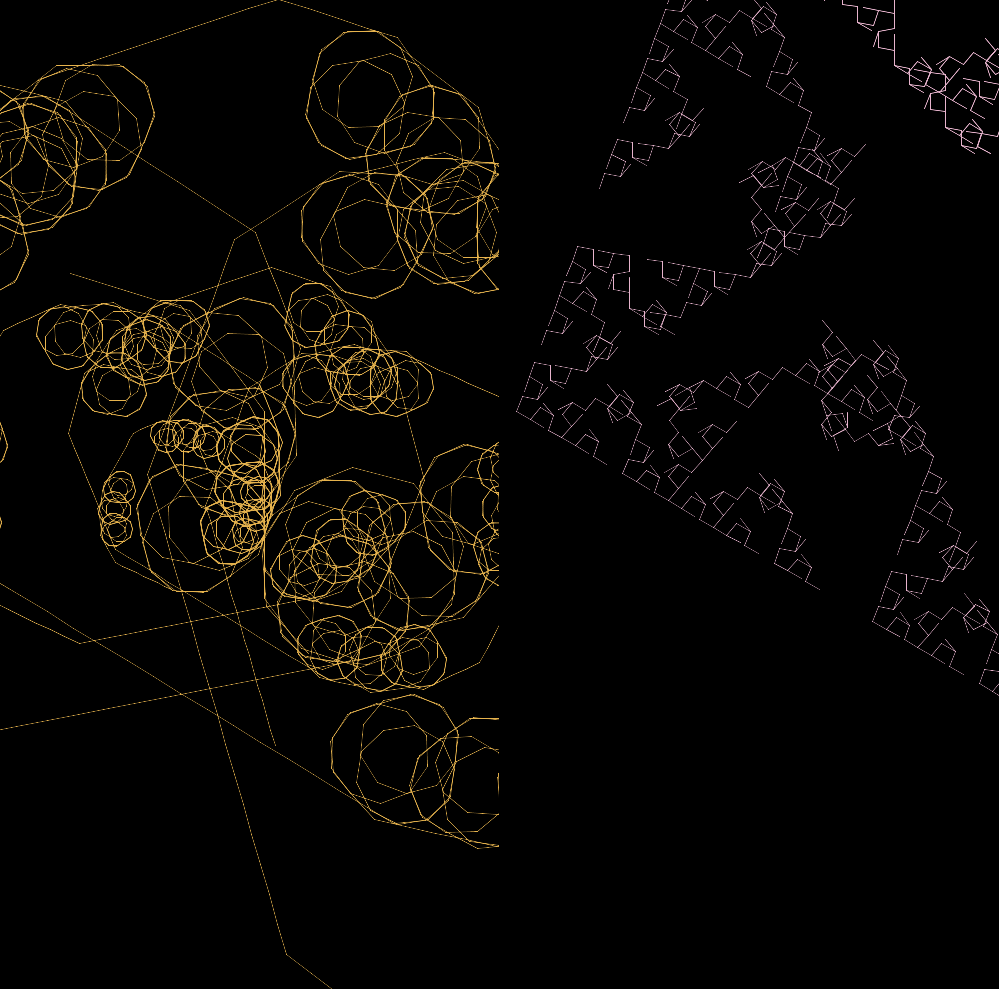
\includegraphics[width=\linewidth]{img/sierpinski_veraestelung_gen8_nebeneinander2x1.png}
\caption{Achte Generation: Die beiden L-Systeme entstehen nebeneinander (eigene Darstellung)}
\label{sierpinski_veraestelung_gen8_nebeneinander2x1}
\end{figure}

Zuletzt wird noch eine Kooperation "`Übereinander"' dargestellt. Für Abbildung \ref{materia_farctal_veraestelung_ueberraschung_uebereinander_gen5} wird zunächst das Partikelsystem geladen und dann werden drei L-Systeme darüber gelagert: Fractal, Verästelung und Überraschung.

\begin{figure}[H]
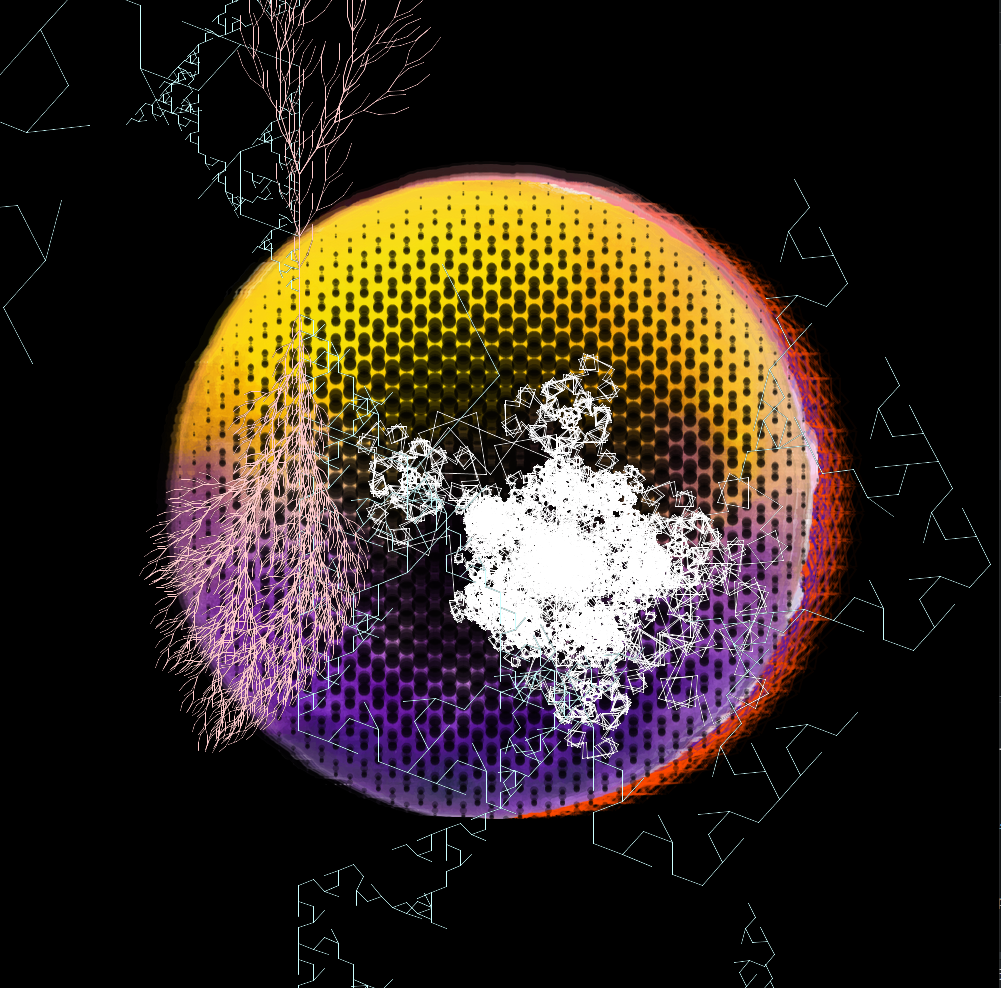
\includegraphics[width=\linewidth]{img/materia_farctal_veraestelung_ueberraschung_uebereinander_gen5.png}
\caption[Kooperation übereinander]{Fünfte Generation: Aus der schwarzen Materie heraus entstehen die beiden L-Systeme, dem Rand der Implosion entwächst ein Baum (eigene Darstellung)}
\label{materia_farctal_veraestelung_ueberraschung_uebereinander_gen5}
\end{figure}

%\bibliographystyle{babplain}
%\bibliography{../mciLiteratur}
\end{document}